\section{Clock and reset strategy}

\subsection{Clocking scheme}

There will be two clock domains, the high and the low-frequency. The low part will operate at 1 MHz and the high at 100 MHz.

\begin{itemize}[nosep]
    \item \textbf{Clock Domains}: The low-frequency components operate across two clock domains:
    \begin{itemize}[nosep]
        \item \textbf{System clock (clk)}: Governs the high-frequency part of the system.
        \item \textbf{Serial clock (sck)}: Operates at up to 1 MHz, driving transaction timing for SPI data input (i\_mosi) and output (o\_miso), sourced from the external SPI Master.
    \end{itemize}
    \item \textbf{Sources}: The system clock (clk) is provided by the internal system, while sck is an external input from the SPI Master.
\end{itemize}

\subsection{Clock Domain Crossings (CDCs)}

For the clock domain crossing there will be 3 main components: 2-flop synchronizers for 1-bit command signals, handshake system with register for data going from low to high-frequency and an asynchronous FIFO for data coming from high to low-frequency. 
Fig.~\ref{fig:cdc-blcok} shows the block diagram for the 3 main components and the signals that are going to cross clock domains.
That are 2 command signals passing through the 2-flop synchronizer, a 16-bit data signal going from low to high-frequency and another 16-bit signal going from the high to low-frequency domain.

\begin{figure}[!htb]
    \centering
    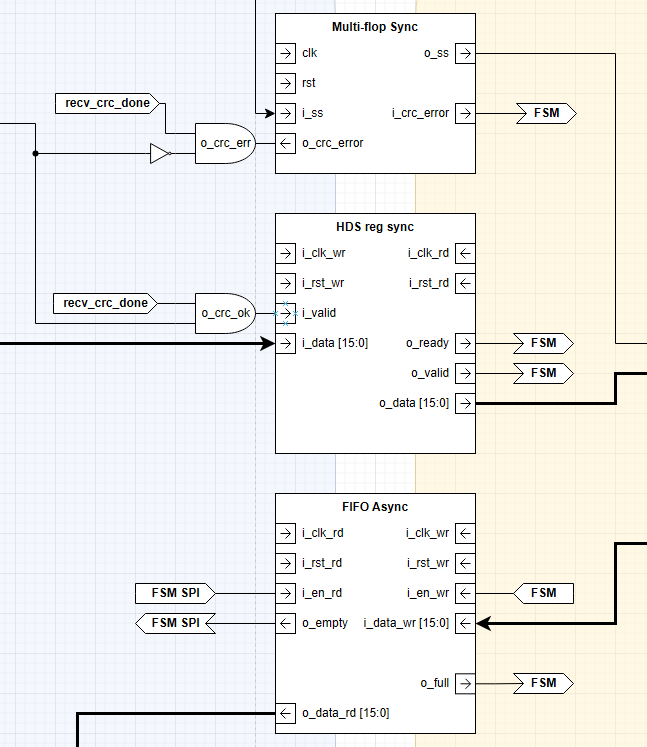
\includegraphics[width=0.5\linewidth]{figures/cdc_block.png}
    \caption{Dual flip-flop synchronizer}
    \label{fig:cdc-blcok}
\end{figure}

Fig.~\ref{fig:ffd-sync} shows the block diagram for the 2-flop synchronizer.

\begin{figure}[!htb]
    \centering
    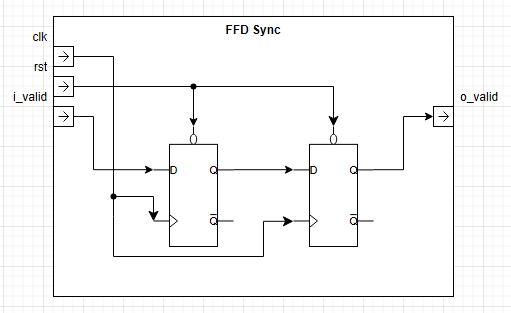
\includegraphics[width=0.5\linewidth]{figures/FFD_sync.png}
    \caption{Dual flip-flop synchronizer}
    \label{fig:ffd-sync}
\end{figure}

Fig.~\ref{fig:hds-reg} shows the block diagram for a handshake register that will be used to transfer the 16-bit data from low to high-frequency.
The handshake with only one register was chosen for this situation because the high-frequency domain will be able to process the data much faster than the low-frequency will be able to receive and transmit the data.

\begin{figure}[!htb]
    \centering
    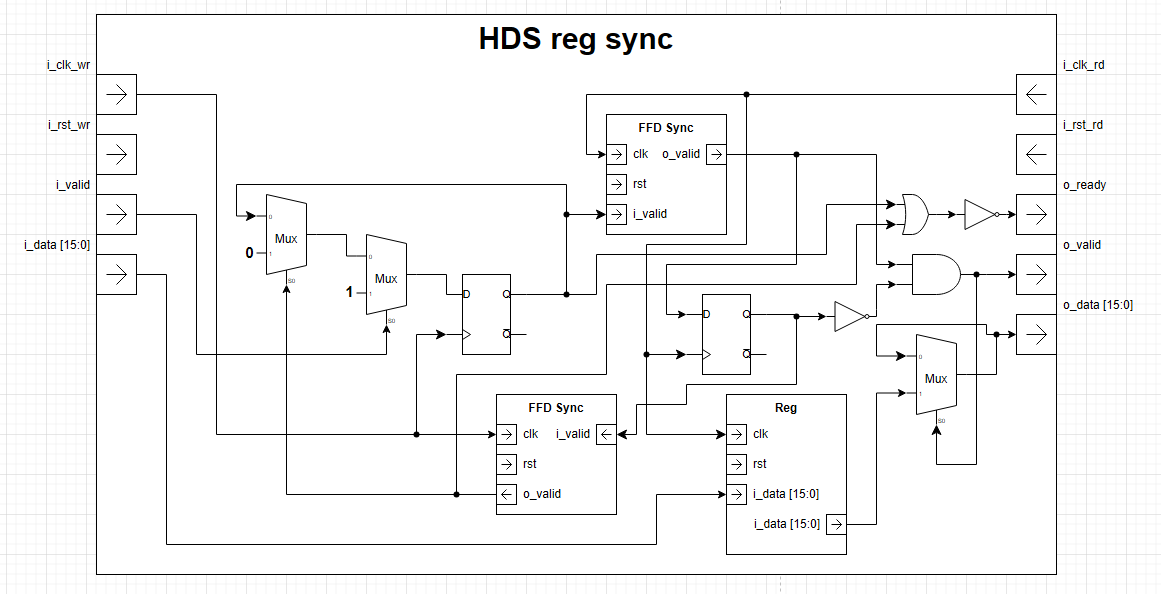
\includegraphics[width=0.5\linewidth]{figures/hds_reg.png}
    \caption{Handshake register}
    \label{fig:hds-reg}
\end{figure}

Fig.~\ref{fig:async-fifo} shows the block diagram for an asynchronous FIFO used to transmit 16-bit data from the high to low-frequency.
The FIFO is needed here because the high-frequency will process and transmit data much faster than the low-frequency, so the buffer is needed to not lose the data and to free the high-frequency domain to do other tasks.

\begin{figure}[!htb]
    \centering
    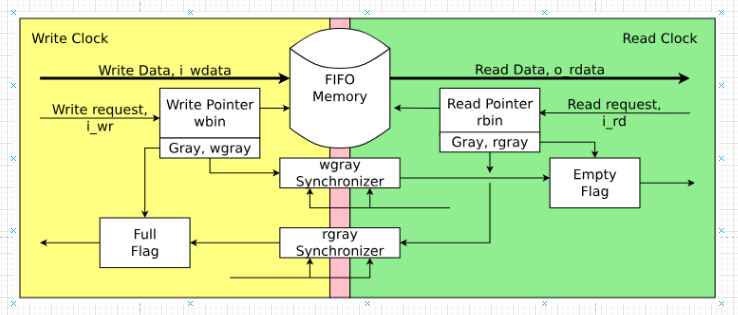
\includegraphics[width=0.5\linewidth]{figures/async_FIFO.png}
    \caption{Asynchronous FIFO}
    \label{fig:async-fifo}
\end{figure}

The designs for these block were inspired by Clifford E. Cummings.

% Signals crossing between sck and clk domains, such as data transitions at the SPI Slave Interface or spi\_busy status, will use synchronization mechanisms like 2-flop synchronizers or handshake protocols to ensure reliable data transfer. Specific CDC implementations will be detailed during RTL design.

\subsection{Reset strategy}

\begin{itemize}[nosep]
    \item \textbf{Reset Signal}: A system reset signal (reset), active low, is used across all blocks in both low-frequency (up to 1 MHz) and high-frequency (100 MHz) domains.
    \item \textbf{Type}: Implements an asynchronous assert phase and synchronous deassert phase to prevent glitches during reset transitions, ensuring reliable initialization of all control and data paths.
    \item \textbf{Implementation Across Clock Domains}: The use of a single reset signal across two clock domains (clk for high-frequency and sck for low-frequency) is chosen for simplicity in design and to ensure global initialization consistency throughout the system. This approach minimizes the complexity of managing multiple reset signals and guarantees that all components start from a known state simultaneously.
    \item \textbf{Synchronous Deassert Phase Clock}: The synchronous deassert phase of the reset signal is governed by the system clock 'clk' (operating at 100 MHz) for consistency in the high-frequency domain. This clock is selected as it is the primary internal system clock, providing better timing control and precision for synchronization, ensuring a clean transition out of reset for critical high-frequency operations.
    \item \textbf{Cross-Domain Synchronization Mechanisms}: To prevent adverse effects such as metastability when the reset signal propagates to the low-frequency domain (sck at up to 1 MHz), synchronization circuits like dual flip-flop synchronizers are employed. These synchronizers ensure that the reset signal is safely aligned with the sck clock domain, avoiding timing mismatches or glitches that could disrupt SPI communication or data integrity during initialization.
\end{itemize}

% \textbf{Reset Signal Propagation Diagram}: Fig.~\ref{fig:reset-sync} illustrates the propagation and synchronization of the reset signal across clock domains, showing the transition from the high-frequency domain (clk) through synchronization logic to the low-frequency domain (sck). This visual aid clarifies how the reset signal is managed to ensure robust system initialization in a multi-domain environment.

% \begin{figure}[!htb]
%     \centering
%     \includegraphics[width=0.5\linewidth]{figures/reset_sync.png}
%     \caption{Reset Signal Synchronization Across Clock Domains}
%     \label{fig:reset-sync}
% \end{figure}
    
\subsection{Architectural Clock Gating}

No architectural clock gating is currently planned for power savings. If power optimization becomes a priority, enable conditions for clock gates can be explored in future design iterations.

% No architectural clock gating is currently planned for power savings in the low-frequency components due to the continuous operation requirement during SPI transactions. If power optimization becomes a priority, enable conditions for clock gates can be explored in future design iterations.
